\PassOptionsToPackage{table}{xcolor}
\documentclass[12pt,letterpaper,twocolumn,openany,nodeprecatedcode,bg=none]{dndbook}
\usepackage[english]{babel}
\usepackage[utf8]{inputenc}
\usepackage{longtable,booktabs,array}
\usepackage{calc}
\usepackage{etoolbox}
\usepackage{caption}
\usepackage{float}
\usepackage{graphicx}
\usepackage{needspace}
\usepackage{tikz}

% Reset zebra striping at the start of every table
\AtBeginEnvironment{longtable}{\rowcolors{1}{white}{gray!10}\small}
\AtBeginEnvironment{table}{\rowcolors{1}{white}{gray!10}}

\providecommand{\pandocbounded}[1]{#1}
\providecommand{\tightlist}{%
  \setlength{\itemsep}{0pt}\setlength{\parskip}{0pt}}

\captionsetup{labelformat=empty}
\setcounter{secnumdepth}{0}
\setlength{\parindent}{0pt}
\setlength{\parskip}{0.5\baselineskip}
\setlength{\headheight}{15pt}

% Prevent orphaned subsections
\let\oldsubsection\subsection
\renewcommand{\subsection}[1]{%
  \needspace{5\baselineskip}%
  \oldsubsection{#1}%
}

\begin{document}
\onecolumn

      \title{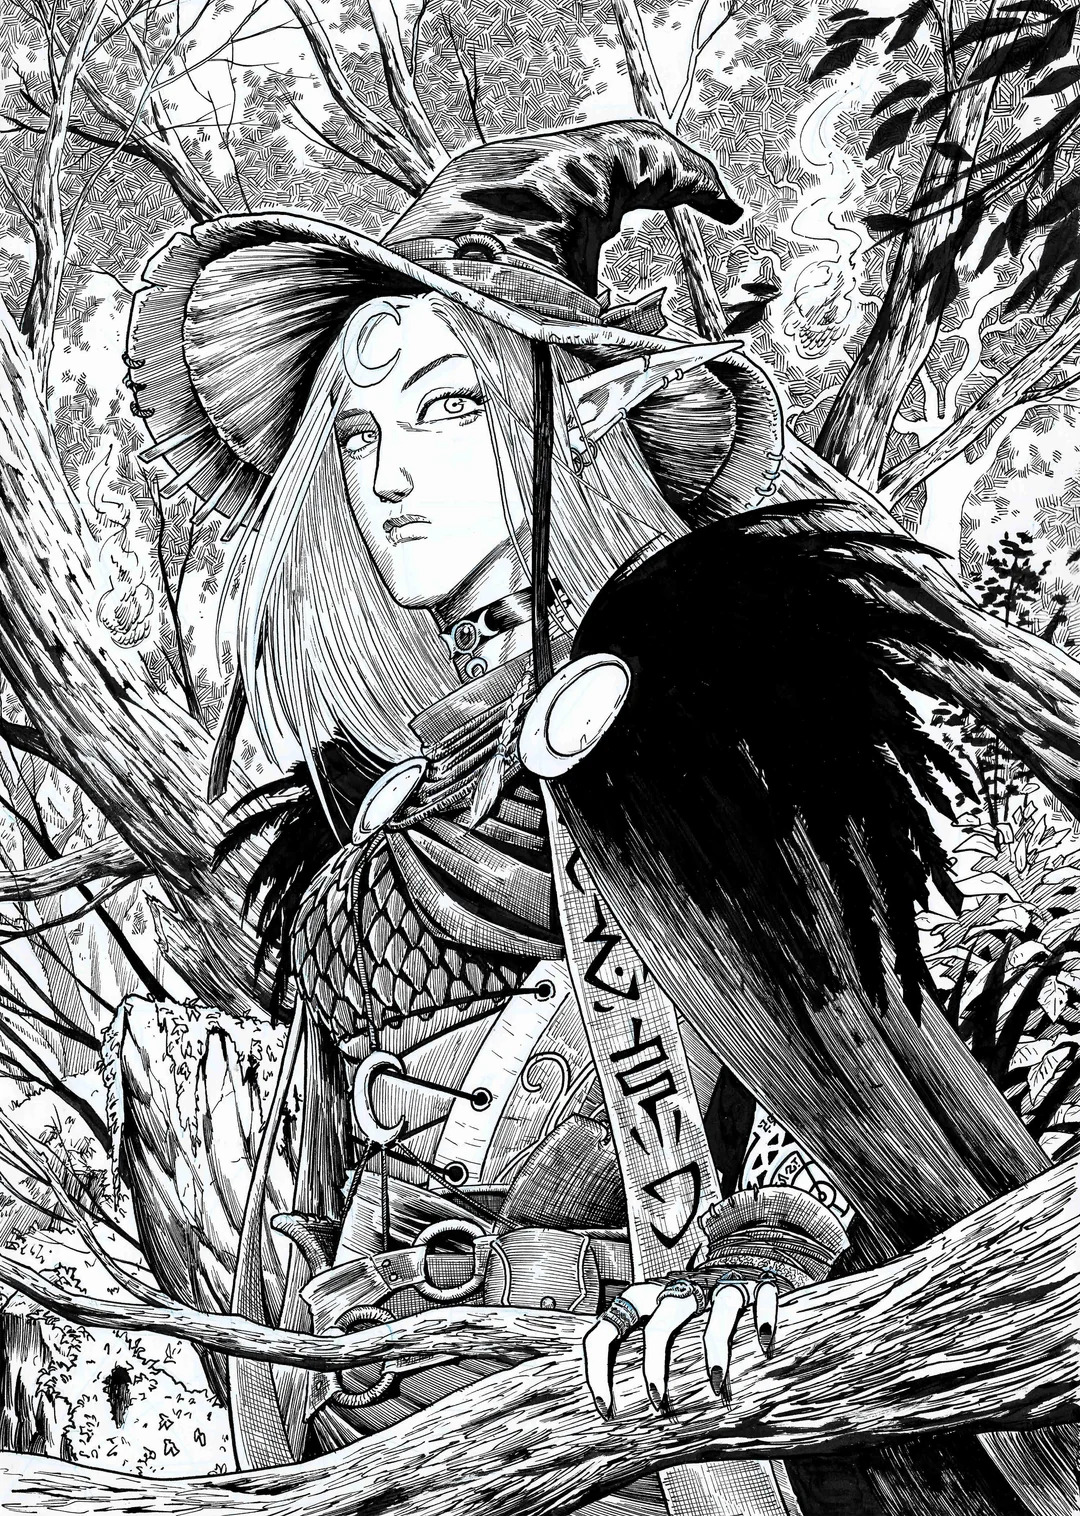
\includegraphics[width=0.9\textwidth,height=0.55\textheight,keepaspectratio]{moonMystic.jpg}\\[1.5cm]Mystic
of the Moon}
  \author{Class Handbook}
\date{}
\maketitle



\clearpage
\twocolumn

\section{Mystic (Moon)}\label{mystic-moon}

\subsection{Core Mystic (Moon) Traits}\label{core-mystic-moon-traits}

\needspace{11\baselineskip}

{\def\LTcaptype{none} % do not increment counter
\begin{table}[!htbp]
\centering
\begin{tabular}{@{}
  >{\raggedright\arraybackslash}p{(\linewidth - 2\tabcolsep) * \real{0.3714}}
  >{\raggedright\arraybackslash}p{(\linewidth - 2\tabcolsep) * \real{0.6286}}@{}}
\toprule\noalign{}
\begin{minipage}[b]{\linewidth}\raggedright
\textbf{Primary Ability}
\end{minipage} & \begin{minipage}[b]{\linewidth}\raggedright
Wisdom
\end{minipage} \\
\midrule\noalign{}
\textbf{Hit Points} & 1d6 \\
\textbf{Saving Throw Proficiencies} & Intelligence, Wisdom \\
\textbf{Skill Proficiencies} & Choose 2 skills \\
\textbf{Weapon Proficiencies} & Choose 1 category \\
\textbf{Starting Equipment} & Breastplate, Handaxe, Dagger, Moonstone
Ring \\
\bottomrule\noalign{}
\end{tabular}
\end{table}
}

\subsection{Mystic (Moon) Features}\label{mystic-moon-features}

\needspace{20\baselineskip}

{\def\LTcaptype{none} % do not increment counter
\begin{table}[!htbp]
\centering
\begin{tabular}{@{}
  >{\raggedright\arraybackslash}p{(\linewidth - 4\tabcolsep) * \real{0.0847}}
  >{\raggedright\arraybackslash}p{(\linewidth - 4\tabcolsep) * \real{0.1864}}
  >{\raggedright\arraybackslash}p{(\linewidth - 4\tabcolsep) * \real{0.7288}}@{}}
\toprule\noalign{}
\begin{minipage}[b]{\linewidth}\raggedright
Level
\end{minipage} & \begin{minipage}[b]{\linewidth}\raggedright
Proficiency
\end{minipage} & \begin{minipage}[b]{\linewidth}\raggedright
Class Features
\end{minipage} \\
\midrule\noalign{}
1 & +2 & Spellcasting, Shape Water, Lunar Navigation \\
2 & +2 & --- \\
3 & +2 & Ability Bonus \\
4 & +2 & --- \\
5 & +2 & Control Water \\
6 & +2 & --- \\
7 & +2 & Ability Bonus \\
8 & +2 & --- \\
9 & +3 & Lunar Shape \\
10 & +3 & --- \\
\bottomrule\noalign{}
\end{tabular}
\end{table}
}

\subsection{Level 1: Spellcasting}\label{level-1-spellcasting}

You can cast spells from the Mystic (Moon) spell list. Wisdom is your
casting ability. You know two cantrips.

You prepare a number of spells equal to your total number of spell
slots. You may change your prepared spells after an extended period of
downtime.

You regain all expended spell slots when you finish a long rest. Once
per day, you may regain 1 expended spell slot when you finish a short
rest.

\subsection{Spell Slots by Level}\label{spell-slots-by-level}

\needspace{20\baselineskip}

{\def\LTcaptype{none} % do not increment counter
\begin{table}[!htbp]
\centering
\begin{tabular}{@{}
  >{\raggedright\arraybackslash}p{(\linewidth - 6\tabcolsep) * \real{0.3571}}
  >{\raggedright\arraybackslash}p{(\linewidth - 6\tabcolsep) * \real{0.2143}}
  >{\raggedright\arraybackslash}p{(\linewidth - 6\tabcolsep) * \real{0.2143}}
  >{\raggedright\arraybackslash}p{(\linewidth - 6\tabcolsep) * \real{0.2143}}@{}}
\toprule\noalign{}
\begin{minipage}[b]{\linewidth}\raggedright
Level
\end{minipage} & \begin{minipage}[b]{\linewidth}\raggedright
1
\end{minipage} & \begin{minipage}[b]{\linewidth}\raggedright
2
\end{minipage} & \begin{minipage}[b]{\linewidth}\raggedright
3
\end{minipage} \\
\midrule\noalign{}
1 & 2 & -- & -- \\
2 & 2 & -- & -- \\
3 & 3 & -- & -- \\
4 & 3 & -- & -- \\
5 & 4 & 2 & -- \\
6 & 4 & 2 & -- \\
7 & 4 & 3 & -- \\
8 & 4 & 3 & -- \\
9 & 4 & 3 & 2 \\
10 & 4 & 3 & 2 \\
\bottomrule\noalign{}
\end{tabular}
\end{table}
}

\subsection{Level 1: Shape Water}\label{level-1-shape-water}

As an action, choose a 5-foot cube of water you can see within 30 feet.
You shape it in one of the following ways:

\begin{itemize}
\tightlist
\item
  \textbf{Part.} You push the water aside, creating a 5-foot-wide,
  5-foot-deep trench for 1 minute.
\item
  \textbf{Raise or Lower.} You raise or lower the water's level by up to
  2 feet.
\item
  \textbf{Move.} You move the water up to 5 feet in any direction.
\item
  \textbf{Freeze.} You freeze a 5-foot square of the water's surface for
  1 minute.
\end{itemize}

\subsection{Level 1: Lunar Navigation}\label{level-1-lunar-navigation}

You can see in moonlight as well as daylight and you can never lose your
orientation as long as you can see the moon and stars.

\subsection{Level 3: Ability Bonus}\label{level-3-ability-bonus}

You gain a +1 bonus to two different abilities of your choice.

\subsection{Level 5: Control Water}\label{level-5-control-water}

Your Shape Water feature improves to have a range of 120 feet and affect
a cube of water up to 30 feet.

\subsection{Level 7: Ability Bonus}\label{level-7-ability-bonus}

You gain a +1 bonus to two different abilities of your choice.

\subsection{Level 9: Lunar Shape}\label{level-9-lunar-shape}

As an action, you can assume a fluid, moonlit form for 1 minute. While
in this form, you gain the following benefits:

\begin{itemize}
\tightlist
\item
  \textbf{Swim Speed.} A swim speed equal to your walking speed.
\item
  \textbf{Waterbreathing.} Can breathe water in addition to air.
\item
  \textbf{Fluid.} Can move through spaces as narrow as 1 inch.
\item
  \textbf{Frost Breath.} As an action, exhale a 30-foot-cone of freezing
  mist. Creatures in the area must make a Constitution save, taking 4d8
  cold damage on a failure or half as much on a success.
\end{itemize}

Once you use this feature, you can't use it again until you finish a
long rest.

\subsection{Mystic (Moon) Spells}\label{mystic-moon-spells}

The tables are numbered for random spell selection.

\subsubsection{Cantrips}\label{cantrips}

\needspace{9\baselineskip}

{\def\LTcaptype{none} % do not increment counter
\begin{table}[!htbp]
\centering
\begin{tabular}{@{}
  >{\raggedright\arraybackslash}p{(\linewidth - 2\tabcolsep) * \real{0.1579}}
  >{\raggedright\arraybackslash}p{(\linewidth - 2\tabcolsep) * \real{0.8421}}@{}}
\toprule\noalign{}
\begin{minipage}[b]{\linewidth}\raggedright
d4
\end{minipage} & \begin{minipage}[b]{\linewidth}\raggedright
Cantrip
\end{minipage} \\
\midrule\noalign{}
1 & Light \\
2 & Minor Illusion \\
3 & Prestidigitation \\
4 & Ray of Frost \\
\bottomrule\noalign{}
\end{tabular}
\end{table}
}

\subsubsection{Level 1 Spells}\label{level-1-spells}

\needspace{13\baselineskip}

{\def\LTcaptype{none} % do not increment counter
\begin{table}[!htbp]
\centering
\begin{tabular}{@{}
  >{\raggedright\arraybackslash}p{(\linewidth - 2\tabcolsep) * \real{0.2000}}
  >{\raggedright\arraybackslash}p{(\linewidth - 2\tabcolsep) * \real{0.8000}}@{}}
\toprule\noalign{}
\begin{minipage}[b]{\linewidth}\raggedright
d6
\end{minipage} & \begin{minipage}[b]{\linewidth}\raggedright
Level 1
\end{minipage} \\
\midrule\noalign{}
1 & Bless \\
2 & Cure Wounds \\
3 & Detect Magic \\
4 & Guiding Bolt \\
5 & Mage Armor \\
6 & Wall of Fog \\
\bottomrule\noalign{}
\end{tabular}
\end{table}
}

\subsubsection{Level 2 Spells}\label{level-2-spells}

\needspace{13\baselineskip}

{\def\LTcaptype{none} % do not increment counter
\begin{table}[!htbp]
\centering
\begin{tabular}{@{}
  >{\raggedright\arraybackslash}p{(\linewidth - 2\tabcolsep) * \real{0.1500}}
  >{\raggedright\arraybackslash}p{(\linewidth - 2\tabcolsep) * \real{0.8500}}@{}}
\toprule\noalign{}
\begin{minipage}[b]{\linewidth}\raggedright
d6
\end{minipage} & \begin{minipage}[b]{\linewidth}\raggedright
Level 2
\end{minipage} \\
\midrule\noalign{}
1 & Augury \\
2 & Hold Creature \\
3 & Mirror Image \\
4 & Restorative Touch \\
5 & See Invisibility \\
6 & Silence \\
\bottomrule\noalign{}
\end{tabular}
\end{table}
}

\subsubsection{Level 3 Spells}\label{level-3-spells}

\needspace{9\baselineskip}

{\def\LTcaptype{none} % do not increment counter
\begin{table}[!htbp]
\centering
\begin{tabular}{@{}
  >{\raggedright\arraybackslash}p{(\linewidth - 2\tabcolsep) * \real{0.1667}}
  >{\raggedright\arraybackslash}p{(\linewidth - 2\tabcolsep) * \real{0.8333}}@{}}
\toprule\noalign{}
\begin{minipage}[b]{\linewidth}\raggedright
d4
\end{minipage} & \begin{minipage}[b]{\linewidth}\raggedright
Level 3
\end{minipage} \\
\midrule\noalign{}
1 & Remove Curse \\
2 & Revivify \\
3 & Speak with Dead \\
4 & Water Breathing \\
\bottomrule\noalign{}
\end{tabular}
\end{table}
}

\newpage

\section{Mystic (Moon) Spell List}\label{mystic-moon-spell-list}

Spells descriptions are listed below.

\subsection{Augury}\label{augury}

\textbf{Level:} 2

You receive an omen from mystical forces about the results of a course
of action that you plan to take within the next 30 minutes. The DM
chooses whether to answer weal, woe, or a mix of the two, depending on
the most likely outcome of the action.

\subsection{Bless}\label{bless}

\textbf{Level:} 1

\textbf{Range:} 30 feet

\textbf{Duration:} Concentration, up to 1 minute

You bless up to three creatures within range. A blessed creature adds
1d4 to their attack rolls and saves.

\subsection{Cure Wounds}\label{cure-wounds}

\textbf{Level:} 1

\textbf{Range:} Touch

A creature you touch regains 2d8 + your spellcasting bonus hit points.

The healing increases to 4d8 + your spellcasting bonus if you use a
level 2 slot and 6d8 + your spellcasting bonus if you use a level 3
slot.

\subsection{Detect Magic}\label{detect-magic}

\textbf{Level:} 1

\textbf{Range:} Self

\textbf{Duration:} Concentration, up to 10 minutes

You see the presence of magical effects within 30 feet on objects that
are visible to you. Magic appears as a faint aura, the details of which
allow you to determine its origin and the basic details of its effect.

\subsection{Guiding Bolt}\label{guiding-bolt}

\textbf{Level:} 1

\textbf{Range:} 120 feet

\textbf{Duration:} 1 round

You hurl a bolt of light toward a creature within range. Make a ranged
spell attack against the target. On a hit, it takes 4d6 radiant damage
and the next attack against the target gains advantage.

The damage increases to 6d6 radiant damage if you use a level 2 slot and
8d6 radiant damage if you use a level 3 slot.

\subsection{Hold Creature}\label{hold-creature}

\textbf{Level:} 2

\textbf{Range:} 60 feet

\textbf{Duration:} Concentration, up to 1 minute

Choose a creature that you can see within range. The target must succeed
on a Wisdom saving throw or become paralyzed. At the end of each of its
turns, the target repeats the save, ending the spell on itself on a
success.

If you use a level 3 slot to cast this spell, you can target two
creatures.

\subsection{Light}\label{light}

\textbf{Level:} Cantrip

\textbf{Range:} Touch

\textbf{Duration:} 1 hour

An object you touch sheds dim light in a 30-foot radius and Dim Light
for an additional 20 feet. The spell ends if you cast it again.

\subsection{Mage Armor}\label{mage-armor}

\textbf{Level:} 1

\textbf{Range:} Touch

\textbf{Duration:} 8 hours

You touch a creature. Until the spell ends, the target can treat its AC
as 13 + its Dexterity modifier.

\subsection{Minor Illusion}\label{minor-illusion}

\textbf{Level:} Cantrip

\textbf{Range:} 30 feet

\textbf{Duration:} 1 minute

You create a sound or an image of an object within range that lasts for
the duration. See the descriptions below for the effects of each. The
illusion ends if you cast this spell again.

A creature can determine that it is an illusion with a successful
Intelligence (Investigation) check against your spell save DC.

\textbf{Sound.} If you create a sound, its volume can range from a
whisper to a scream that can last up to the spell's duration.

\textbf{Image.} An image you create cannot be larger than a 5-foot cube
or a size Medium creature. The image can't create sound, light, smell,
or any other sensory effect. Physical interaction with the image reveals
it to be an illusion.

\subsection{Mirror Image}\label{mirror-image}

\textbf{Level:} 2

\textbf{Range:} Self

\textbf{Duration:} 1 minute

Three illusory duplicates of yourself appear in your space. The
duplicates move with you and mimic your actions, shifting position so
it's impossible to track which image is real.

Each time a creature hits you with an attack roll during the spell's
duration, roll a d6 for each of your remaining duplicates. If any of the
d6s rolls a 3 or higher, one of the duplicates is hit instead of you,
and the duplicate is destroyed. The duplicates otherwise ignore all
other damage and effects. The spell ends when all three duplicates are
destroyed.

A creature is unaffected by this spell if it cannot see or can use other
senses to pinpoint you.

\subsection{Prestidigitation}\label{prestidigitation}

\textbf{Level:} Cantrip

\textbf{Range:} 10 feet

\textbf{Duration:} Up to 1 hour

You create a minor magical effect within range. You can light a torch,
create a glowing sigil, clean off an object, or create an object that
can fit in the palm of your hand. An object created in this manner is an
obvious, worthless duplicate. The spell ends if you cast it again.

\newpage

\subsection{Ray of Frost}\label{ray-of-frost}

\textbf{Level:} Cantrip

\textbf{Range:} 60 feet

A frigid beam of blue-white light streaks toward a creature within
range. Make a ranged spell attack against the target. On a hit, it takes
1d8 cold damage, and its speed is reduced by 20 feet until after its
next turn.

The damage increases to 2d8 cold damage at level 5 and 3d8 cold damage
at level 9.

\subsection{Remove Curse}\label{remove-curse}

\textbf{Level:} 3

\textbf{Range:} Touch

At your touch, all curses affecting one creature or object end. If the
object is a cursed magic item, its curse remains, but the spell allows
the owner to remove or discard it.

\subsection{Restorative Touch}\label{restorative-touch}

\textbf{Level:} 2

\textbf{Range:} Touch

You touch a creature and end one condition on it: blinded, paralyzed, or
poisoned.

\subsection{Revivify}\label{revivify}

\textbf{Level:} 3

\textbf{Range:} Touch

You touch a creature. If that creature died within the last minute, it
returns to life, restores one failed death save, and regains 1 hit
point. It cannot restore failed death saves again until it finishes a
long rest.

\subsection{See Invisibility}\label{see-invisibility}

\textbf{Level:} 2

\textbf{Range:} Self

\textbf{Duration:} 1 hour

You see creatures and objects that are invisible as if they were
visible.

\subsection{Silence}\label{silence}

\textbf{Level:} 2

\textbf{Range:} 120 feet

\textbf{Duration:} Concentration, up to 10 minutes

No sound can be created within or pass through a 20-foot-radius sphere
centered on a point you choose within range. Any creature or object
entirely inside the sphere has immunity to thunder damage. Spells cannot
be cast in the spell's area.

\newpage

\subsection{Speak with Dead}\label{speak-with-dead}

\textbf{Level:} 3

\textbf{Range:} 10 feet

\textbf{Duration:} 10 minutes

You touch a corpse and attempt to commune with its spirit. If its spirit
can be contacted, you contact it through mystical means.

Until the spell ends, you can ask the spirit of the corpse up to five
questions. The spirit knows only what it knew in life, including the
languages it knew. The spirit is under no compulsion to offer a truthful
answer if you are antagonistic toward it or it recognizes you as an
enemy.

The dead often demand a service in return for the information they
provide. If you accept such a deal, you cannot cast this spell again
until you complete the task or make a good faith effort to do so.

\subsection{Wall of Fog}\label{wall-of-fog}

\textbf{Level:} 1

\textbf{Range:} 120 feet

\textbf{Duration:} 10 minutes

You create a thick, billowing wall of fog that blocks sight and sound.
It is one-foot thick, 10 feet high, and up to 30 feet long. The wall can
bend and turn as you wish, but all of it must be within the spell's
range when you create it.

\subsection{Water Breathing}\label{water-breathing}

\textbf{Level:} 3

\textbf{Range:} 30 feet

\textbf{Duration:} 24 hours

This spell grants up to ten willing creatures of your choice within
range the ability to breathe underwater until the spell ends. Affected
creatures also retain their normal mode of respiration.

\onecolumn

\clearpage
\thispagestyle{empty}
\begin{center}
\vspace*{\fill}
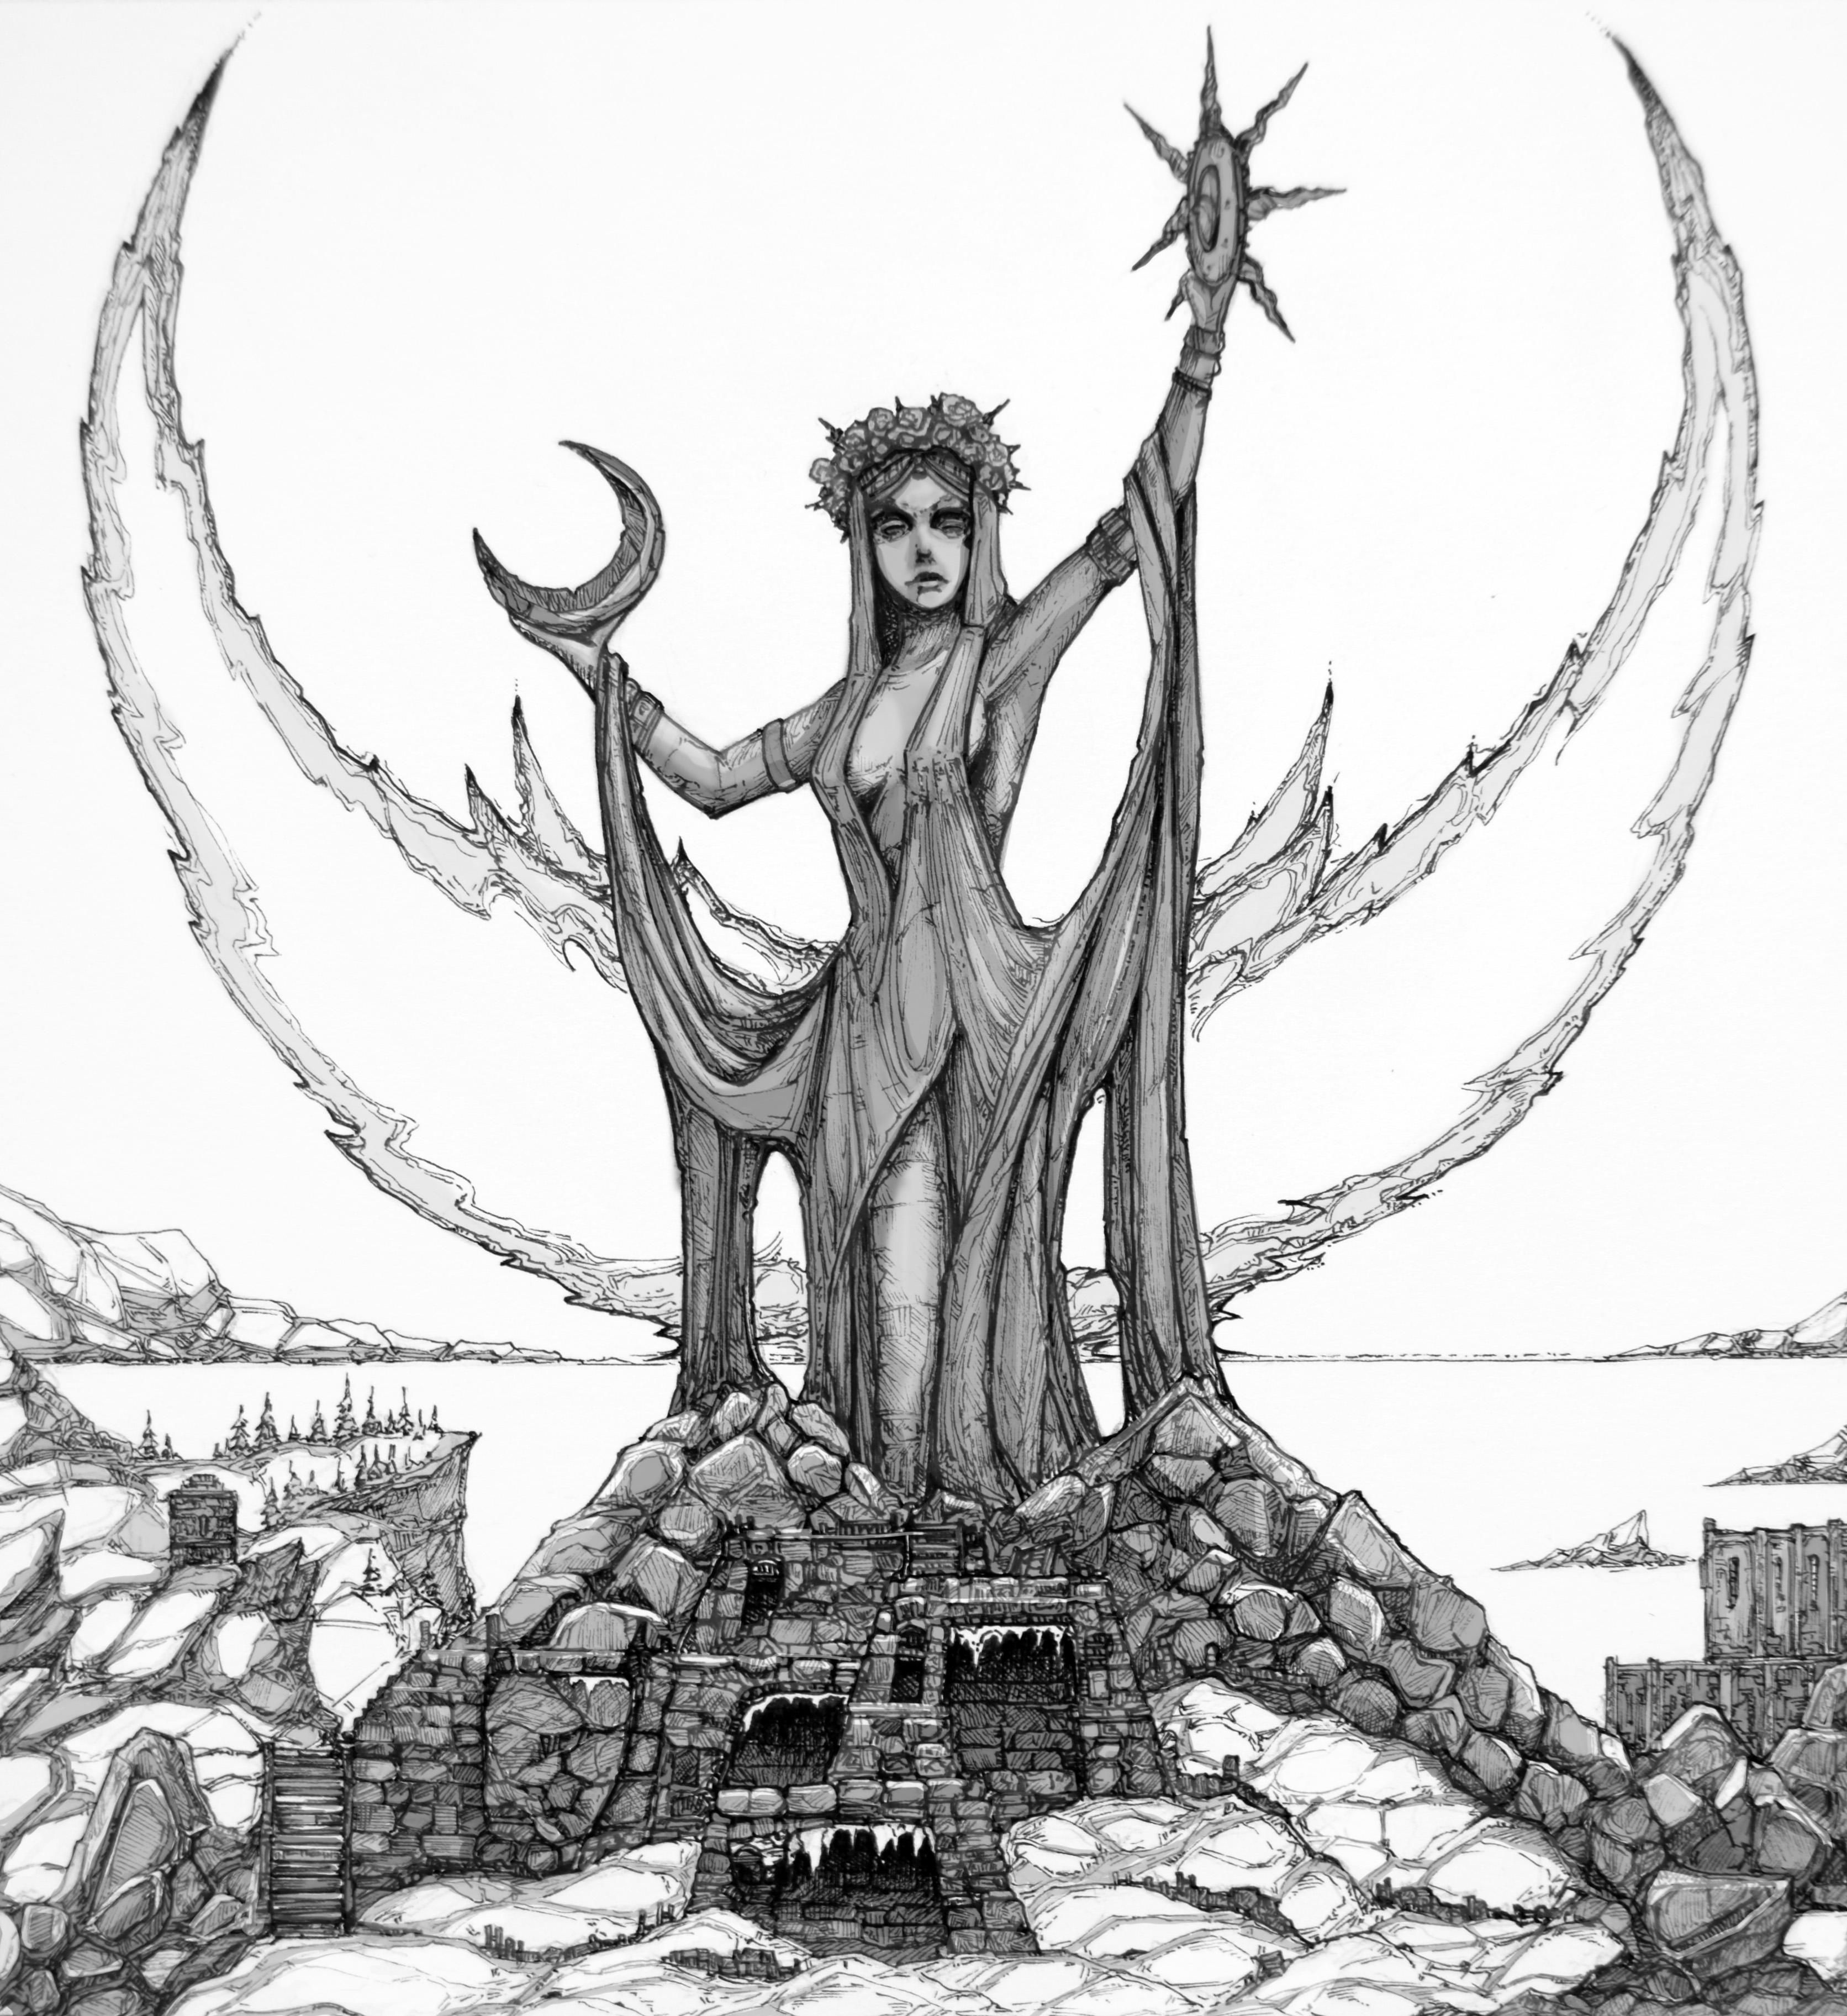
\includegraphics[width=0.7\textwidth,keepaspectratio]{azura-bw.jpg}\par
\vspace{0.4cm}
{\itshape Come moon and star, let us gaze upon the world.}\par
\vspace*{\fill}
\end{center}

\end{document}